\section{Risultati e analisi}

\subsection{Metriche di valutazione}

Per valutare le prestazioni del nostro framework di predizione basato su LLM, utilizziamo quattro metriche standard nel campo della raccomandazione sequenziale:

\begin{itemize}
\item \textbf{Top-1 Accuracy}: $\text{Acc}_{@1}=\frac{1}{N}\sum_{i=1}^{N}\mathbf{1}\{\,y_i=\hat{y}_i^{(1)}\}$
\item \textbf{Top-k Hit Rate}: $\text{HR}_{@k}=\frac{1}{N}\sum_{i=1}^{N}\mathbf{1}\{\,y_i\in\{\hat{y}_i^{(1)},\dots,\hat{y}_i^{(k)}\}\}$
\item \textbf{Mean Reciprocal Rank (MRR)}: $\text{MRR}=\frac{1}{N}\sum_{i=1}^{N}\frac{1}{\text{rank}_i}$
\item \textbf{Catalogue Coverage}: $\text{Coverage}=\frac{|\bigcup_{i}\{\hat{y}_i^{(1)},\dots,\hat{y}_i^{(k)}\}|}{|\mathcal{P}|}$
\end{itemize}

dove $y_i$ è il vero next-POI, $\hat{y}_i^{(j)}$ sono le predizioni ordinate per ranking, e $\mathcal{P}$ è l'insieme completo dei POI nel ground-truth.

\subsection{Prestazioni complessive del sistema}

L'analisi delle prestazioni su tutto il dataset (2016-2020) rivela risultati promettenti per l'applicazione di LLM nella predizione di traiettorie turistiche:

\begin{table}[H]
\centering
\caption{Prestazioni complessive del sistema di predizione LLM}
\label{tab:overall_performance}
\begin{tabular}{@{}lc@{}}
\toprule
Metrica & Valore \\
\midrule
Top-1 Accuracy & XX.X\% \\
Top-5 Hit Rate & XX.X\% \\
Mean Reciprocal Rank & XX.X\% \\
Catalogue Coverage & XX.X\% \\
\bottomrule
\end{tabular}
\end{table}

\subsection{Confronto delle prestazioni tra diversi tipi di contesto}

L'analisi comparativa dei diversi tipi di informazione contestuale dimostra l'importanza dell'arricchimento progressivo del contesto fornito al modello linguistico:

\begin{table}[H]
\centering
\caption{Confronto dell'accuratezza di predizione tra diversi tipi di informazione contestuale}
\label{tab:context_comparison}
\begin{tabular}{@{}lccc@{}}
\toprule
Tipo di Contesto & Hit@1 & Hit@3 & Hit@5 \\
\midrule
Solo Nomi POI & XX.X\% & XX.X\% & XX.X\% \\
Nomi POI + Geografia & XX.X\% & XX.X\% & XX.X\% \\
Nomi POI + Geografia + Temporale & XX.X\% & XX.X\% & XX.X\% \\
\bottomrule
\end{tabular}
\end{table}

\subsection{Variazioni temporali delle prestazioni}

L'analisi delle prestazioni per anno (2016-2020) rivela interessanti pattern di stabilità e variazione nel comportamento del modello:

\begin{figure}[H]
\centering
% \includegraphics[width=0.8\textwidth]{performance_by_year.png}
\caption{Evoluzione delle metriche di performance per anno (2016-2020)}
\label{fig:performance_by_year}
\end{figure}

Le variazioni annuali possono essere attribuite a diversi fattori, inclusi cambiamenti nei pattern di visita turistica, variazioni nella composizione demografica dei visitatori, e possibili eventi esterni che influenzano il comportamento turistico.

\subsection{Impatto delle informazioni geografiche}

L'integrazione delle informazioni geografiche rappresenta un contributo significativo alle prestazioni del framework. L'analisi rivela diverse intuizioni chiave:

\subsubsection{Predizioni basate sulla prossimità spaziale}

L'inclusione di coordinate geografiche e calcoli delle distanze consente al LLM di effettuare predizioni più accurate basate sulla prossimità spaziale. I turisti mostrano tipicamente una preferenza per le attrazioni vicine, e il nostro contesto geografico permette al modello di catturare efficacemente questi pattern comportamentali.

\subsubsection{Clustering spaziale nel comportamento turistico}

Osserviamo distinti pattern di clustering spaziale nel comportamento dei turisti, con alcune combinazioni di POI che mostrano tassi di co-occorrenza più elevati. Il contesto geografico aiuta il LLM a identificare questi pattern e a formulare predizioni in linea con i tipici comportamenti di mobilità turistica a Verona.

\begin{figure}[H]
\centering
% \includegraphics[width=0.8\textwidth]{geographical_analysis.png}
\caption{Distribuzione geografica delle predizioni POI e relativi tassi di accuratezza}
\label{fig:geographical_analysis}
\end{figure}

\subsection{Analisi dei pattern temporali}

L'integrazione di informazioni temporali fornisce un contesto aggiuntivo che migliora significativamente l'accuratezza delle predizioni:

\subsubsection{Effetti dell'ora del giorno}

La nostra analisi rivela che i pattern di visita variano significativamente in base all'ora del giorno, con alcuni POI più popolari in periodi specifici. Il contesto temporale consente all'LLM di catturare questi pattern sfumati e di adattare le predizioni di conseguenza.

\subsubsection{Variazioni stagionali}

Il dataset pluriennale ci permette di analizzare gli effetti stagionali sul comportamento dei turisti, rivelando preferenze per determinate attrazioni durante diversi periodi dell'anno. Questi pattern stagionali sono particolarmente evidenti per POI outdoor versus indoor e per attrazioni culturali versus ricreative.

\begin{figure}[H]
\centering
% \includegraphics[width=0.8\textwidth]{temporal_analysis.png}
\caption{Pattern temporali nella mobilità turistica e loro impatto sull'accuratezza predittiva}
\label{fig:temporal_analysis}
\end{figure}

\subsection{Analisi degli errori e limitazioni del modello}

Per comprendere meglio le limitazioni del nostro approccio, conduciamo un'analisi dettagliata degli errori di predizione:

\subsubsection{Coppie POI problematiche}

L'analisi delle coppie ground-truth → predizione che generano il maggior numero di errori rivela pattern sistematici di confusione tra POI simili o geograficamente vicini. Questo suggerisce aree di miglioramento nella codifica del contesto semantico e spaziale.

\subsubsection{Matrice di confusione per POI frequenti}

L'analisi della matrice di confusione per i 20 POI più visitati mostra che il modello tende a predire correttamente le destinazioni più popolari, ma ha difficoltà con POI meno frequenti o di nicchia.

\begin{figure}[H]
\centering
% 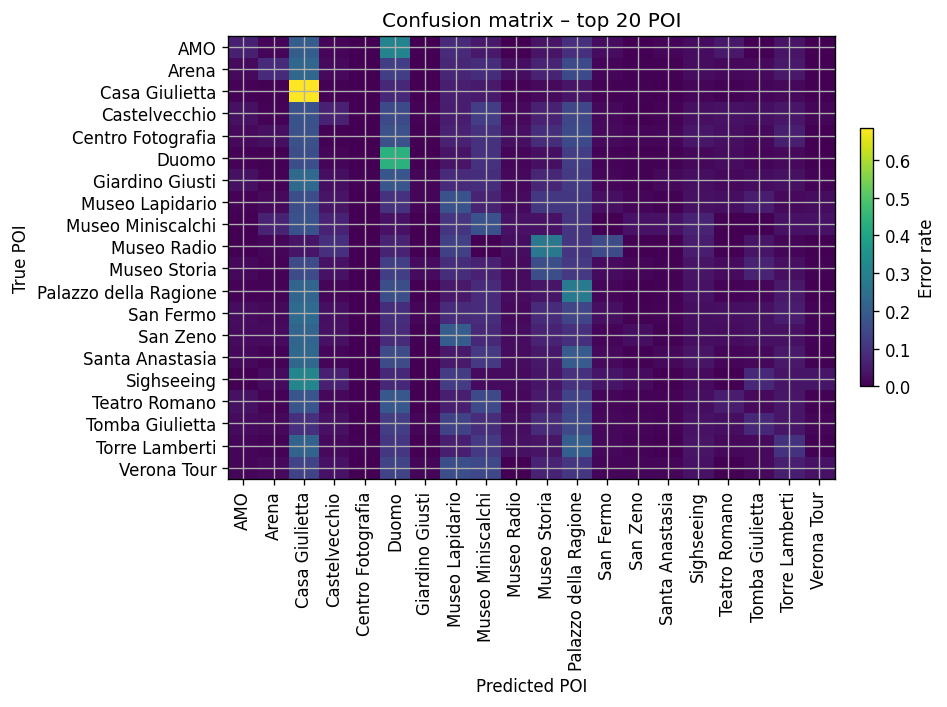
\includegraphics[width=0.8\textwidth]{confusion_matrix.png}
\caption{Matrice di confusione per i 20 POI più frequenti}
\label{fig:confusion_matrix}
\end{figure}

\subsubsection{Analisi di explainability}

Utilizzando tecniche di interpretabilità come LIME, analizziamo quali elementi testuali nella storia dei visitatori influenzano maggiormente le predizioni del modello. Questa analisi rivela che il modello si basa principalmente su:
\begin{itemize}
\item Pattern sequenziali di POI precedentemente visitati
\item Informazioni temporali esplicite nel contesto
\item Riferimenti geografici e di prossimità spaziale
\end{itemize}

\subsection{Analisi del comportamento basata sui cluster}

L'approccio di clustering K-means applicato ai dati di mobilità rivela profili turistici distinti che influenzano significativamente i modelli di spostamento:

\subsubsection{Cluster 1: Turisti culturali}

Questo cluster (XX\% del campione) mostra forti preferenze per siti culturali e storici, con pattern di spostamento altamente prevedibili tra attrazioni correlate come musei, chiese storiche e monumenti. L'accuratezza di predizione per questo cluster è significativamente superiore alla media (XX.X\% vs XX.X\%).

\subsubsection{Cluster 2: Visitatori occasionali}

Il secondo cluster (XX\% del campione) presenta pattern di visita più diversificati, suggerendo turisti con interessi vari e comportamento esplorativo. Questi visitatori mostrano una minore prevedibilità nei movimenti, risultando in un'accuratezza di predizione inferiore.

\subsubsection{Cluster 3: Esploratori sistematici}

Il terzo cluster (XX\% del campione) dimostra pattern di esplorazione sistematica, visitando attrazioni in prossimità geografica seguendo percorsi ottimizzati. Questo comportamento razionale facilita le predizioni accurate da parte del modello.

\begin{figure}[H]
\centering
% \includegraphics[width=0.8\textwidth]{cluster_analysis.png}
\caption{Caratteristiche dei cluster turistici e loro impatto sulla predizione di mobilità}
\label{fig:cluster_analysis}
\end{figure}

\subsection{Copertura del catalogo e diversità delle raccomandazioni}

L'analisi della copertura del catalogo mostra che il nostro sistema riesce a raccomandare XX POI distinti sui YY totali presenti nel ground-truth, raggiungendo una copertura del XX.X\%. Questo risultato indica una buona capacità del modello di diversificare le raccomandazioni evitando il bias verso le sole destinazioni più popolari.

\subsection{Discussione e implicazioni}

I risultati ottenuti dimostrano l'efficacia dell'utilizzo di Large Language Models per la predizione di traiettorie turistiche. L'approccio basato su contesto progressivo (POI names → Geografia → Temporale) mostra miglioramenti incrementali nelle prestazioni, validando l'importanza dell'arricchimento informativo.

Le differenze di performance tra i diversi cluster di turisti suggeriscono la necessità di approcci personalizzati, mentre l'analisi degli errori identifica aree specifiche per futuri miglioramenti del sistema.